\documentclass{beamer}
\usepackage{beamerthemesplit}
\usepackage{subfig}
\usepackage{amssymb,amsmath,mathtools}
\usepackage{amsfonts,booktabs}
\usepackage{lmodern,textcomp}
\usepackage{color}
\usepackage{tikz}
\usepackage{natbib}
\usepackage{multicol}
\usepackage{ctex}
\usepackage[level]{datetime}
\usepackage{listings}


\usetheme{Warsaw}
\newdateformat{ukdate}{\monthname[\THEMONTH] \ordinaldate{\THEDAY} , \THEYEAR}
\lstset{
 columns=fixed,       
 numbers=left,                                        % 在左侧显示行号
 numberstyle=\tiny\color{gray},                       % 设定行号格式
 frame=none,                                          % 不显示背景边框
 backgroundcolor=\color[RGB]{245,245,244},            % 设定背景颜色
 keywordstyle=\color[RGB]{40,40,255},                 % 设定关键字颜色
 numberstyle=\footnotesize\color{darkgray},           
 commentstyle=\it\color[RGB]{0,96,96},                % 设置代码注释的格式
 stringstyle=\rmfamily\slshape\color[RGB]{128,0,0},   % 设置字符串格式
 showstringspaces=false,                              % 不显示字符串中的空格
 language=c++,                                        % 设置语言
}


\title{基于生成式先验的人像视频编辑}
\author{汪兆辰}
\date{\ukdate\today}

\begin{document}

\begin{frame}
    \titlepage
\end{frame}

\section{总体设想}

\begin{frame}
    \frametitle{总体设想}
    基于文章Portait Video Editing Empowered by MultiModal Generative Priors
    提出的方法,开发一个Web客户端实现对用户上传的人像视频的编辑,包括:
    \begin{itemize}
        \item 文字驱动的视频编辑
        \item 图像驱动的视频编辑
        \item 改变全局光照
    \end{itemize}
\end{frame}

\begin{frame}
    \begin{itemize}
        \item 更进一步地,该工作使用了多种先验模型:在对人体建模时使用了SMPL-X;而由于文章中提出的视频生成策略
    为使用2D生成模型迭代更新视频帧数据集,再调整3DGS渲染出结果,因此可以考虑替换效果更好的先验模型,以
    提高视频编辑的效率和质量。
    
        \item 另一方面,在文章的演示中,该方法主要被应用于风格化处理视频和衣着替换,可以考虑
    开发更多的功能。
    \end{itemize}
\end{frame}

\section{目前进展}

\begin{frame}
    \begin{itemize}
        \frametitle{目前进展}
        \item 正在学习MIT Web Development课程,预计本周完成,之后将着手搭建网站基本架构。
        \item 调研了一些相关最新文献,考虑在后续添加新功能
    \end{itemize}
\end{frame}

\section{问题}

\begin{frame}
    \frametitle{问题}
    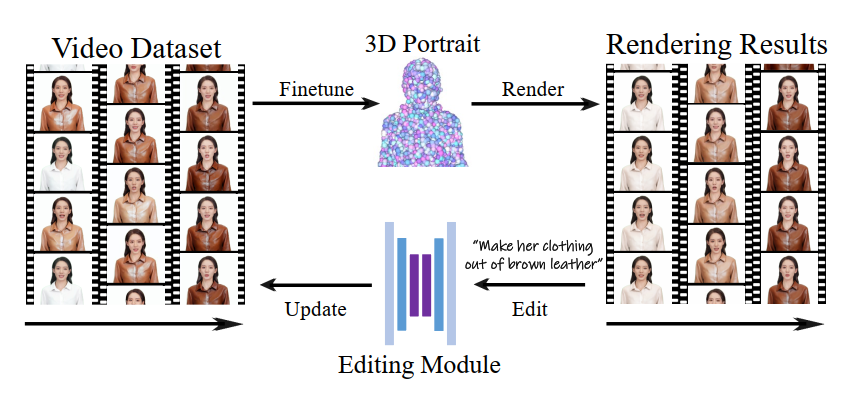
\includegraphics[width=\textwidth]{pic1.png}
\end{frame}


\end{document}